\documentclass[spanish]{textolivre}

% metadata
\journalname{Texto Livre}
\thevolume{18}
%\thenumber{1} % old template
\theyear{2025}
\receiveddate{\DTMdisplaydate{2024}{1}{19}{-1}}
\accepteddate{\DTMdisplaydate{2024}{2}{21}{-1}}
\publisheddate{\today}
\corrauthor{Carmen Llorente-Cejudo}
\articledoi{10.1590/1983-3652.2025.49561}
%\articleid{NNNN} % if the article ID is not the last 5 numbers of its DOI, provide it using \articleid{} commmand 
% list of available sesscions in the journal: articles, dossier, reports, essays, reviews, interviews, editorial
\articlesessionname{articles}
\runningauthor{Cabero-Almenara, Rodríguez Gallego, Llorente-Cejudo}
%\editorname{Leonardo Araújo} % old template
\sectioneditorname{Daniervelin Pereira}
\layouteditorname{Leonardo Araújo}

\title{Realidad mixta, virtual y aumentada: tecnologías para el aprendizaje}
\othertitle{Realidade mista, virtual e aumentada: tecnologias para aprendizagem}
\othertitle{Mixed, virtual and augmented reality: technologies for learning}

\author[1]{Julio Cabero-Almenara~\orcid{0000-0002-1133-6031}\thanks{Email: \href{mailto:cabero@us.es}{cabero@us.es}}}
\author[1]{Margarita Rodríguez Gallego~\orcid{0000-0001-6959-4829}\thanks{Email: \href{mailto:margaguez@us.es}{margaguez@us.es}}}
\author[1]{Carmen Llorente-Cejudo~\orcid{0000-0002-4281-928X}\thanks{Email: \href{mailto:karen@us.es}{karen@us.es}}}
\affil[1]{Universidad de Sevilla, Facultad de Ciencias de la Educación, Departamento de Didáctica y Organización Educativa, Sevilla, España.}

\addbibresource{article.bib}

\usepackage{multirow}

\begin{document}
\maketitle
\begin{polyabstract}
\begin{abstract}
La potencialidad que las herramientas como la Realidad Aumentada, la Realidad Virtual o la Realidad Mixta poseen, tanto a nivel tecnológico como didáctico, ha hecho que los centros educativos las incorporen atendiendo a dos de sus características distintivas: accesibilidad y relevancia. En el artículo que se presenta, se analiza a través de una revisión exhaustiva de estudios, investigaciones y metaanálisis, las diferentes posibilidades didácticas que estos recursos ofrecen para el ámbito educativo. Asimismo, se analizan las diferentes líneas de investigación que se están desarrollando con el objetivo de ampliar el conocimiento científico disponible, entre las que se pueden destacar algunas como: formación del profesorado para su uso didáctico; búsqueda de principios para el diseño de objetos de aprendizaje; grado de aceptación y actitudes que despiertan en docentes y estudiantes; percepciones sobre las dificultades a la hora de incorporarlas; variables cognitivas asociadas a su utilización; o, estudios comparativos para conocer su eficacia, entre otras.

\keywords{Realidad mixta \sep Realidad virtual \sep Realidad aumentada \sep Aprendizaje}
\end{abstract}

\begin{portuguese}
\begin{abstract}
O potencial que ferramentas como Realidade Aumentada, Realidade Virtual ou Realidade Mista possuem, tanto a nível tecnológico como didático, fez com que os centros educativos as incorporassem com base em duas das suas características distintivas: acessibilidade e relevância. Neste artigo, são analisadas as diferentes possibilidades didáticas que esses recursos oferecem para o campo educacional por meio de uma revisão exaustiva de estudos, pesquisas e meta-análises. Da mesma forma, são analisadas as diferentes linhas de pesquisa que estão sendo desenvolvidas com o objetivo de ampliar o conhecimento científico disponível, dentre as quais se destacam algumas como: formação de professores para uso didático; busca de princípios para o design de objetos de aprendizagem; grau de aceitação e atitudes que despertam em professores e alunos; percepções sobre as dificuldades ao incorporá-las; variáveis cognitivas associadas ao seu uso; estudos comparativos para conhecer sua eficácia, entre outros.

\keywords{Realidade mista \sep Realidade virtual \sep Realidade aumentada \sep Aprendizado}
\end{abstract}
\end{portuguese}

\begin{english}
\begin{abstract}
The potential that tools such as Augmented Reality, Virtual Reality or Mixed Reality possess, both at a technological and didactic level, has made educational centers incorporate them based on two of their distinctive characteristics: accessibility and relevance. In the article presented, the different didactic possibilities that these resources offer for the educational field are analyzed through an exhaustive review of studies, research and meta-analysis. Likewise, the different lines of research that are being developed are analyzed with the aim of expanding the available scientific knowledge, among which some can be highlighted such as: teacher training for didactic use; search for principles for the design of learning objects; degree of acceptance and attitudes that they awaken in teachers and students; perceptions about the difficulties when incorporating them; cognitive variables associated with its use; or, comparative studies to know its effectiveness, among others.

\keywords{Mixed reality \sep Virtual reality \sep Augmented reality \sep Learning}
\end{abstract}
\end{english}
\end{polyabstract}

\section{Introducción}
Nunca en la historia de la humanidad, y menos en la historia de la educación, tanto el docente como el discente han contado con tantas tecnologías como en la actualidad. Tecnologías que han sido consideradas por algunos como tecnologías emergentes. Tecnologías que de acuerdo con \textcite[p.~13]{cabero_2023}, vienen caracterizadas por tres aspectos: “a) son herramientas e innovaciones metodológicas, b) experimentan un ciclo de sobre expectativa y c) pueden ser potencialmente disruptivas.” Una de estas tecnologías, aunque desde nuestra perspectiva no cumple la tercera característica apuntada, son las tecnologías de la Realidad Aumentada (RA - Augmented Reality), la Realidad Virtual (RV - Virtual Reality) y la Realidad Extendida (RE - extended reality) o Mixta; tecnologías que permiten, por lo general, la incorporación de la persona a entornos desarrollados a través de imágenes reales (vídeos, imágenes, vídeos en 360º, ...) o artificiales (imágenes en 2D, imágenes en 3D, imágenes generadas mediante Inteligencia Artificial, ...), que permiten la inmersión de la persona en esos contextos.

Esta situación ha sido potenciada por una serie de hechos, como son: 

\begin{enumerate}
    \item La fuerza que presentan las nuevas computadoras para ofrecer con calidad y realismo la información audiovisual y multimedia, que son claves en la utilización de estos recursos inmersivos que trataremos en el presente artículo; 
    \item La velocidad de procesamiento de la información que ofrecen las nuevas computadoras, que depende de diferentes variables (velocidad del procesador, la arquitectura del procesador, la capacidad de la memoria RAM, ...), las características del nuevo software de producción de estos objetos que están apareciendo en el mercado (Layar, Zappar, Krpano, ...), la mayor disponibilidad de los teléfonos celulares en la población, o la disminución de los costos de los equipos que se utilizan tanto para la producción como para el visionado de los recursos.
\end{enumerate}

El conjunto de influencias anteriormente apuntadas, han propiciado que las tecnologías que analizamos sean señaladas por diferentes autores e informes \cite{brown_2020,joosten2020digital,kukulska-hulme2021innovating,pelletier2021educause}, con una marcada tendencia hacia su integración en el ámbito educativo en un futuro próximo. Independientemente de la disciplina o el nivel de estudio, que su incorporación pueda manifestarse de manera independiente o en interacción con otras innovaciones tecnológicas, destacan la "Inteligencia Artificial" y el "e-learning".

Tal importancia se observa por el aumento de trabajos de investigación y teóricos sobre las mismas que este hecho está repercutiendo en que diferentes autores estén realizando estudios de metaanálisis sobre los resultados que están ofreciendo las diferentes investigaciones realizadas, lo que facilita a la comunidad investigadora la construcción de un cuerpo teórico, tanto para su utilización como para su diseño y producción \cite{dinatale2020immersive,tang2020evaluating,howard2021meta,yu_2021,roda2022using,Zeeshan_2022,wang2023application}.

Aunque posteriormente se abordará de manera específica la problemática de los resultados encontrados, apuntemos ya que las investigaciones realizadas tienden a presentar resultados positivos y de mejora en diferentes variables, tales como el rendimiento académico, la motivación o el grado de aceptación por los estudiantes cuando se utilizan en acciones formativas. 

Pero, antes de seguir avanzando, dedicar unos momentos a establecer lo que en el presente artículo se van a entender por las tres tecnologías apuntadas, señalando también algunas de sus posibilidades para ser utilizadas en contextos instruccionales, así como determinadas limitaciones y dificultades que se han apuntado para su incorporación a la formación. 

En este sentido, es conveniente asumir desde el principio, como señalan \textcite[p.~1]{rauschnabel2022xr}, que: 

\begin{quote}
La realidad aumentada (AR), la realidad virtual (VR), la realidad mixta y la realidad extendida (a menudo, engañosamente, abreviada como XR) son términos comúnmente utilizados para describir cómo las tecnologías generan o modifican la realidad. Sin embargo, académicos y profesionales han sido inconsistentes en el uso de estos términos. Esto ha llevado a confusión conceptual y demarcaciones poco claras. Inspirándonos en investigaciones previas y conocimientos cualitativos de profesionales de XR, discutimos el significado y las definiciones de varios términos y los organizamos en nuestro marco propuesto.
\end{quote}


Iniciando con la exploración de la RA, es pertinente destacar que esta tecnología faculta la integración de información digital con el entorno físico en tiempo real, utilizando diversos dispositivos tecnológicos como \textit{tablets} o \textit{smartphones}. De este modo, se genera una nueva realidad mediada por dichos dispositivos.

Uno de los trabajos clásicos que se utiliza para diferenciar la RA respecto a otras de las tecnologías abordadas en el presente artículo, es la conceptualización propuesta hace tempo por \textcite{milgram1994taxonomy}, que en el continuo realidad-virtualidad, la RA se posiciona más cercana al contexto físico, mientras que la RV ocupa uno de los extremos. En el punto intermedio, se sitúa la categoría de "Realidad Virtual Aumentada" o "Realidad Extendida o Mixta", la cual incorpora elementos tanto de la RA como de la RV. Este enfoque conceptual proporciona un marco de referencia para comprender las relaciones entre estas tecnologías emergentes.

La distinción entre estas modalidades tecnológicas puede ser observada a través de la propuesta efectuada por \textcite{rauschnabel2022xr} (\Cref{fig1}). Estos autores, al destacar la existencia de cierta ambigüedad conceptual en los términos utilizados, proponen considerar la presencia o ausencia del entorno físico como un criterio fundamental para la conceptualización y diferenciación de dichas modalidades.

\begin{figure}
    \centering
    \begin{minipage}{.85\textwidth}
    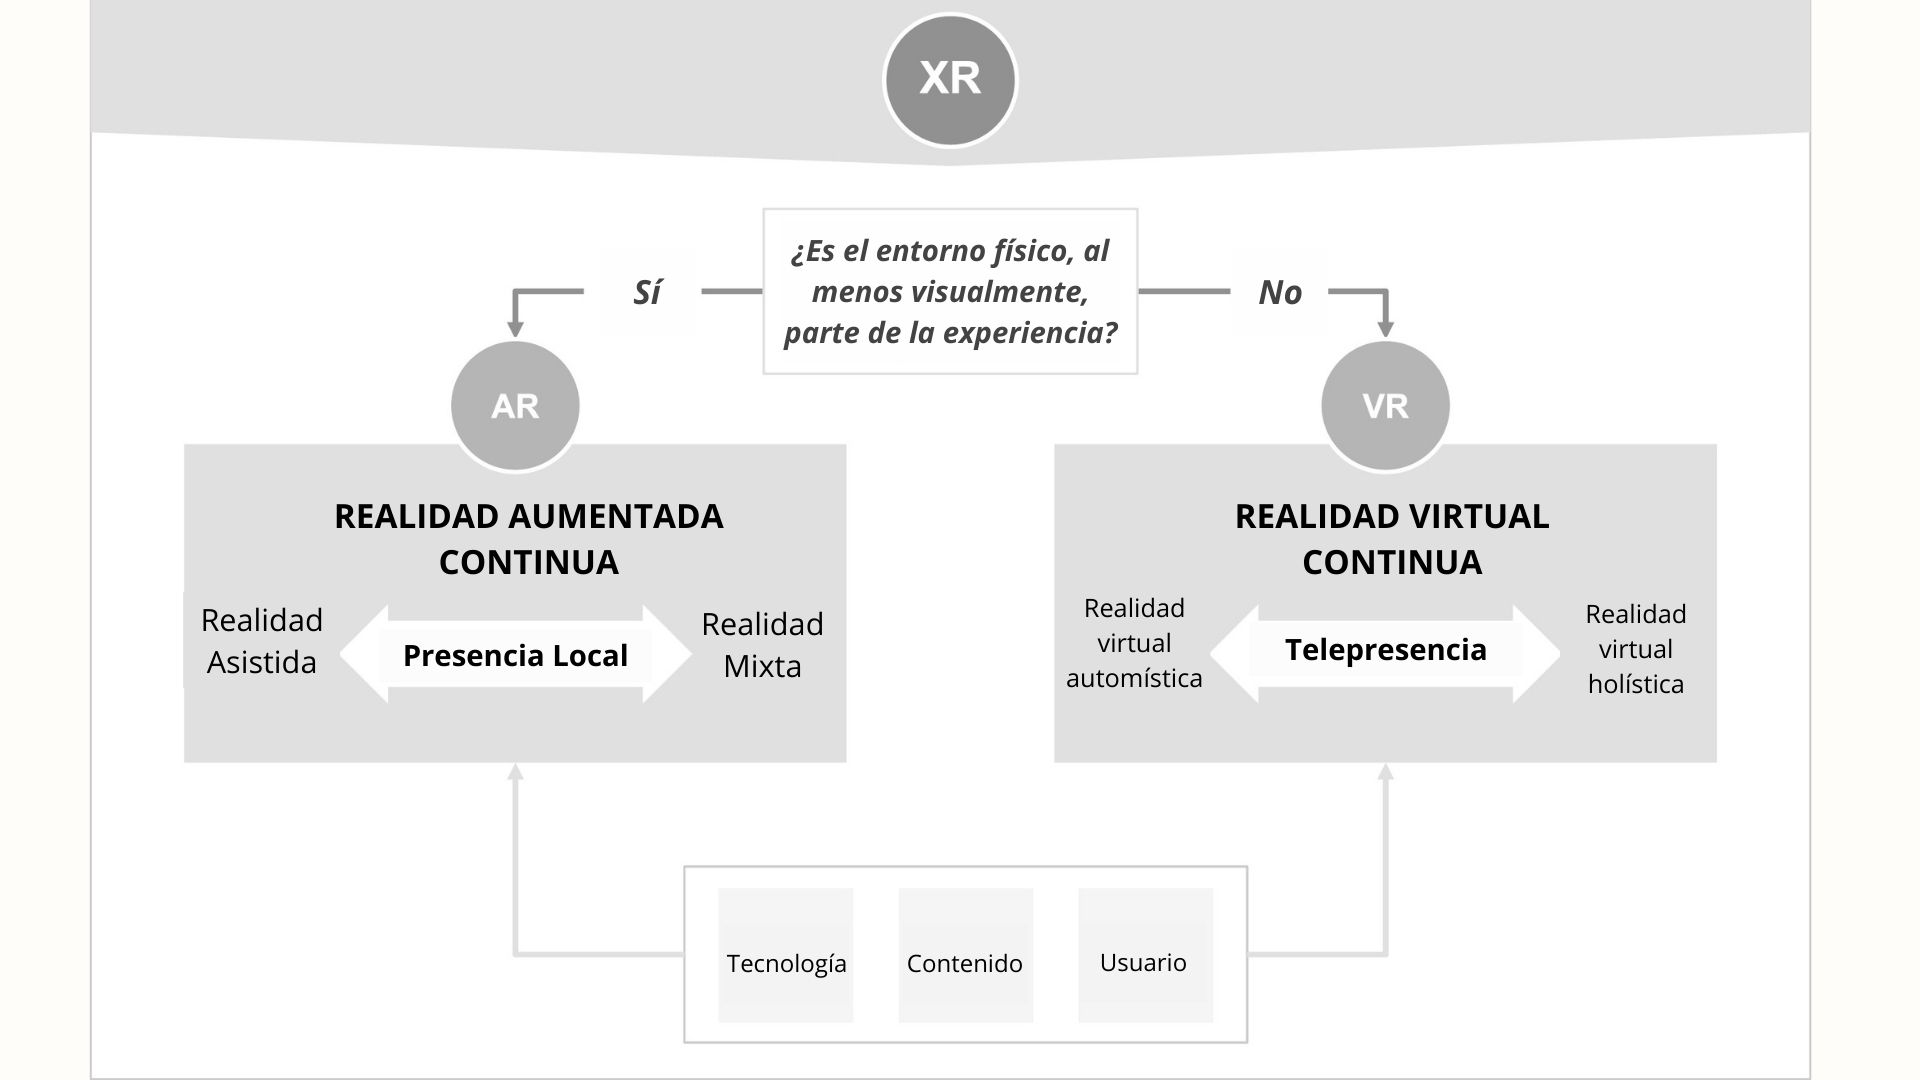
\includegraphics[width=\linewidth]{Fig1.png}
    \caption{Esquema de la realidad mixta o extendida y la realidad aumentada y virtual.}
    \label{fig1}
    \source{\cite[p.~6]{rauschnabel2022xr}}
    \end{minipage}
\end{figure}

 Como apuntaron en su momento \textcite[p.~12]{cabero2022ecosystem}, existe: 

\begin{quote}
una clara diferencia entre la realidad aumentada y virtual, ya que en la segunda, los datos virtuales sustituyen a los físicos, creándose una nueva realidad. Por el contrario, en la realidad aumentada, las dos realidades se superponen en distintas capas de información en formatos diversos (imágenes generadas por ordenador, secuencias de vídeo, animaciones, etc.) para configurar una nueva realidad que es con la que interacciona la persona.
\end{quote}

Las definiciones que se han ofrecido de la Realidad Virtual son diversas, y ya \textcite[p.~1171]{huang2010investigating} apuntaban la siguiente: 

\begin{quote}
un VRLE permite la visualización de datos tridimensionales (3D) y proporciona un entorno interactivo que refuerza la sensación de una inmersión en el mundo virtual generado por un ordenador. Además, una VRLE ofrece la oportunidad de simular un entorno realista y seguro para que los alumnos realicen tareas específicas. Una VRLE ofrece simulación en tiempo real donde se usan gráficos tridimensionales de computadora para imitar el mundo real.
\end{quote}


Conceptualización que como se puede observar con otras más actuales, como por ejemplo la formulada por \textcite{navarro2019realidad}, no han variado mucho en el tiempo, ya que estos autores llegan a entenderla como:

\begin{quote}
un entorno que puede ser de apariencia real o no, que da al usuario la sensación de estar inmerso en él. Como norma general, este entorno es generado por un sistema informático y visualizado por el usuario mediante un dispositivo específico como pueden ser un casco o unas gafas y, dependiendo del sistema y de lo elaborado e inmersivo que pretenda ser, puede estar acompañado de otros elementos como sensores de posición y movimiento, guantes, sonido, elementos como mandos para desplazarse o manipular los objetos del entorno, etc. \cite[p.~37]{navarro2019realidad}
\end{quote}
 

No obstante, es imperativo considerar que dentro del ámbito de la RV coexisten dos variantes claramente definidas: la modalidad inmersiva y la no inmersiva \cite{caballero_2020}. La primera busca crear un entorno tecnológico que lleve al sujeto a sentirse incorporado en un entorno tecnológico, y persigue de esta manera general una experiencia en el sujeto intensa y envolvente. Cada una de estas variantes presenta características particulares; la modalidad inmersiva, por un lado, se distingue por un costo elevado, ofrecer una alta interactividad al sujeto, una complejidad en su utilización, ofrecimiento de gráficos y audio de alta calidad, propensión a inducir desorientación en el usuario, generación de una intensa sensación de realidad, y la provisión de una experiencia de inmersión total. Por otro lado, la modalidad no inmersiva, caracterizada por un costo más accesible, el interfaz con el que interacciona el sujeto es más sencillo, una mayor facilidad de uso, una pronta aceptación por parte de los usuarios, una disminuida sensación de realidad, menor desconexión con el entorno ofrece al sujeto la menor posesión a la desorientación, y una inmersión más parcial, constituye la segunda variante. Cabe destacar que estas variantes han sido conceptualizadas también como inmersivas o de escritorios. 

Distintos académicos han propuesto una clasificación adicional en la RV, segregándola en dos categorías: la RV de baja inmersión, la cual hace uso de dispositivos convencionales como el ratón y el teclado para la interacción, y la de alta inmersión, que típicamente implica la utilización de dispositivos como los visualizadores montados en la cabeza ("Head-Mounted Display" o HMD) \cite{mulders2020framework}.

Por otro lado, diversos estudiosos han propuesto una clasificación tridimensional de los sistemas de RV:

\begin{enumerate}
\item Sistemas Inmersivos, los cuales posibilitan que el usuario experimente una total inserción en el entorno virtual sin mantener contacto alguno con la realidad circundante.
\item Sistemas Semi-inmersivos o de Proyección, caracterizados por la disposición de cuatro pantallas dispuestas en forma de cubo (tres en las paredes y una en el suelo), rodeando al usuario y permitiéndole mantener cierto contacto con elementos del mundo real.
\item Sistemas No-inmersivos o de Escritorio, en los cuales la interfaz de acceso al mundo virtual se limita a una pantalla única \cite{otegui2017realidad}.
\end{enumerate} 
 
En lo que respecta a la distinción entre RA y RV, resulta imperativo considerar que, mientras la RA superpone elementos como imágenes, sonidos, modelos 3D, videos, gráficos, secuencias animadas, juegos e información de GPS generados por computadora sobre entornos del mundo real; la RV constituye una tecnología que posibilita la inmersión del individuo en un espacio de 360º grados, generado en 3D o capturado por cámaras de 360º, facilitando la inmersión en primera persona ya sea en un entorno generado de manera real o virtual.
 
Conforme señalan \textcite{park2022metaverse}, la RA ofrece una solución realista, dada la simplicidad y la habitualidad de los dispositivos utilizados para su ejecución, tales como tabletas, teléfonos inteligentes o gafas, y refleja de manera efectiva la realidad, si bien es más apropiada para contenidos de corta duración. En contraste, la RV abarca todo el campo visual, brinda una sensación de inmersión y presenta el problema adicional de la fatiga cognitiva del usuario, la desorientación y el aumento de la carga cognitiva que debe movilizar el sujeto para desplazarse por el entorno tecnológico.

Creemos que lo apuntado permite que el lector adquiera unas bases sólidas para discriminar entre la RA y RV de todas formas el lector interesado en ampliar la información puede consultar el trabajo realizado por \textcite{rauschnabel2022xr}, que discriminan las diferencias entre ambas realidades en función de distintos aspectos: papel desempeñado por el entorno físico para alcanzar la nueva realidad, el tiempo de uso, contexto de uso típico, tecnología empleada, riesgos físicos y cognitivos para el usuario, problemática de la privacidad, sensación de desorientación y mareo, mecanismos específicos para el visionado y casos típicos de utilización.

Por lo que se refiere a la RE, se debe señalar desde el principio que esta tecnología representa una integración de la RA y la RV. En consecuencia, posibilita la generación de objetos virtuales que facilitan la interacción de los usuarios con el entorno tridimensional. Este proceso se materializa mediante la inmersión en el entorno virtual propio de la RV, a la par que se superponen contenidos virtuales mediante la aplicación de la RA
Como señalan \textcite[p.~29]{brown_2020}: 

\begin{quote}
La realidad extendida (XR) es un término integral para los entornos que combinan lo físico con lo virtual o brindan experiencias virtuales completamente inmersivas. Las dos tecnologías más comunes son la realidad aumentada (AR) y la realidad virtual (VR). Mientras que la RA superpone objetos físicos y lugares con contenido virtual, la RV suele ser una experiencia más inmersiva, que implica manipulaciones e interacciones con objetos virtuales dentro de un entorno completamente virtual.
\end{quote}


Como se muestra, de acuerdo con los comentarios realizados por \textcite{wang2023application}, en la \Cref{fig2}, los tres tipos de realidades comentadas difieren en términos de características de interacción, así en la RV es unidireccional, en la RA es unidireccional y bidireccional y en la RE se permite la interacción bidireccional entre usuarios. y espacios tanto virtuales como físicos.

\begin{figure}
\centering
\begin{minipage}{.85\textwidth}
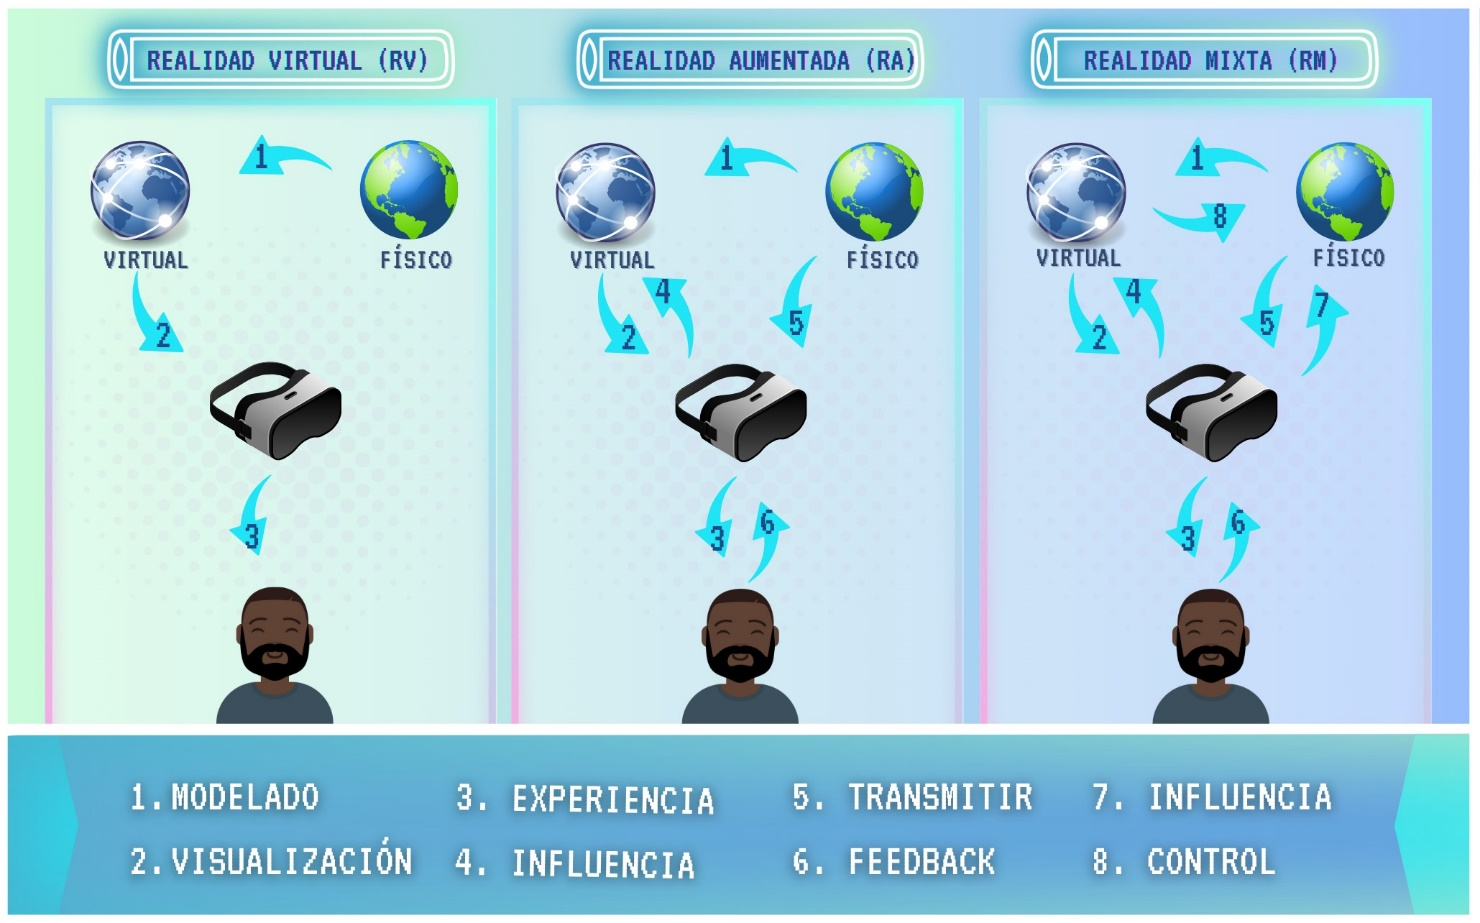
\includegraphics[width=\linewidth]{Fig2.png}
\caption{Identificación de la capacidad de interacción tecnológica.}
\label{fig2}
\source{\cite[p.~755]{ke2019enhanced}}
\end{minipage}
\end{figure}
 
Por su parte, en la \Cref{tbl1}, \textcite[p.~755]{ke2019enhanced} ofrecen un estudio diferenciador de las características distintivas de cada una de las tecnologías que se presentan en nuestro artículo, que puede servirnos a manera de síntesis de lo expuesto hasta el momento.

\begin{table}[htbp]
\caption{Características de las tecnologías de la RV, RA y RE.}
\label{tbl1}
\centering
\begin{tabular}{lllll}
\toprule
Propiedades & Características & RV & RA & RE \\ 
\midrule
\multirow{3}{*}{Inmersión} & Espacio Virtual & X & X & X \\ 
& Espacio Físico & & X & X \\
& Tiempo real de interacción & & & X \\
\multirow{3}{*}{Interactividad} & Usuario y Modelo virtual & X & X & X \\
& Usuario y espacio físico & & X & X \\
& Objetos Físico y Modelo Virtual & & & X \\
\multirow{3}{*}{Percepción Múltiple} & Información Virtual & X & X & X \\
& Información Real & & X & X \\
& Información fisiológica de los usuarios & & X \\
\multirow{5}{*}{Llave tecnológica} & Tecnología de simulación & X & X & X \\
& Tecnología de monitor & X & X & X \\
& Grafismo de ordenador & X & X & X \\
& Interacción tecnológica humano ordenador & & X & X \\
& Tecnología de seguimiento de registro & & X & X \\
\bottomrule
\end{tabular}
\source{\cite[p.~755]{ke2019enhanced}}
\end{table}

En resumen, y siguiendo la propuesta realizada por \textcite{park2022metaverse}, se puede decir que mientras la RV genera una realidad novedosa basada en imágenes de 360 grados, la RA constituye un método para superponer objetos virtuales en el espacio real. En contrapartida, la RE o Mixta se caracteriza por integrar estos dos conceptos previos, facultando a los usuarios para interactuar con el entorno tridimensional mediante la inmersión del entorno virtual de la RV y la superposición de contenido virtual a través de la RA.


\section{¿Qué dice la investigación sobre sus posibilidades educativas?}\label{sec-normas}
Antes de presentar algunos de los resultados alcanzados en las investigaciones, es preciso apuntar cuáles han sido los criterios empleados para la selección de los diferentes estudios e investigaciones que conforman el metaanálisis realizado para desarrollar la justificación teórica del trabajo que se presenta. Y en este sentido, los criterios adoptados han sido varios: por un lado, indicar que son artículos de carácter nacional e internacional basados en estudios e investigaciones publicados en revistas de impacto, en bases de datos tales como Web of Science, Journal Citation Reports (JCR), Scimago Journal and Country Rank (SJR) y SCOPUS. 

Asimismo, se incorpora también como criterio que estas publicaciones hayan presentado un volumen elevado de citación en lo que respecta a los trabajos realizados sobre la temática abordada (RA, RV o Inmersiva, RE), así como la relevancia de los diferentes autores que suscriben las publicaciones en la temática objeto de estudio. 

Por lo tanto, y para comenzar el análisis, lo primero de todo es señalar que las potencialidades educativas atribuidas a las tecnologías mencionadas exhiben variaciones sustanciales entre sí. Esta diversidad es inherentemente lógica, dada la disparidad en los momentos temporales de implementación en el ámbito educativo, la multiplicidad de tecnologías requeridas para su ejecución, el desarrollo de los programas de producción, su fiabilidad para la presentación de la información, los costos asociados a su implantación, su dificultad de utilización, la complejidad de su producción, y los efectos psicológicos que inducen en los individuos que las emplean.

En esta situación es necesario asumir, que cuando hablamos de su aplicación al contexto educativo resulta imperativo reconocer que el conocimiento más amplio respecto a su aplicación educativa se encuentra en la tecnología de RA, seguida por la RV, y finalmente, por la RE o Mixta. Esta última, se halla en una fase incipiente de desarrollo y difusión en las instituciones educativas, con limitadas investigaciones efectuadas, y en ella llegan a sobresalir más sus aplicaciones comerciales y recreativas, que las educativas que se encuentran en su fase de iniciación.

En el contexto de la RA, cabe destacar que uno de los fundamentos que respaldan su aplicación en el ámbito formativo radica en su capacidad para facilitar la comprensión de conceptos complicados. Esta capacidad se sustenta en la posibilidad de visualizar objetos desde diversas perspectivas, así como en la capacidad de descomponer dichos elementos en etapas, fases o partes, lo cual contribuye a una aprehensión más efectiva por parte del estudiante como obtuvimos nosotros en la diversidad de investigaciones que realizamos dentro del proyecto de investigación I+D+i denominado “Realidad Aumentada para Aumentar la Formación. Diseño, Producción y Evaluación de Programas de Realidad Aumentada para la Formación Universitaria”, a las cuales puede acceder el lector interesado en ellas en la página web que se elaboró específicamente para el proyecto. Por otra parte, la RA posibilita la substitución de objetos físicos, especialmente relevantes en disciplinas artísticas y científicas, mediante representaciones digitales más accesibles y seguras para los estudiantes, facilitando de esta forma la manipulación de los objetos con completa tranquilidad. En definitiva, otro aspecto que abona a la consideración de la RA en entornos educativos es su capacidad para propiciar la interactividad de los estudiantes con la información virtual proporcionada. Esta interactividad se manifiesta directamente en la capacidad de los estudiantes para manipular objetos y elementos de manera tangible, prescindiendo de tecnologías complejas y garantizando un entorno seguro para la exploración y aprendizaje.

Iniciando la presentación de algunos de los resultados alcanzados, lo primero que se debe apuntar es que en la gran mayoría de las investigaciones realizadas, por no decir todas, que han analizado el grado de aceptación que despierta en los estudiantes su utilización en la educación analizados con los modelos TAM (Technology Acceptance Model) o UTAUT (Unified Theory of Acceptance and Use of Technology), han indicado que los estudiantes muestran un elevado grado de aceptación para interaccionar con estas tecnologías.

Por otra parte, se debe destacar que diferentes investigaciones han señalado que los estudiantes muestran un alto nivel de participación y satisfacción, cuando se implican en este tipo de experiencias \cite{cabero_2018,cabero2020use}. Esta perspectiva de relevancia no se limita únicamente al momento en que los estudiantes actúan como receptores y usuarios de esta tecnología. Ello también viene impulsado porque los dispositivos básicos de interacción, los teléfonos celulares despiertan un verdadero grado de aceptación en los estudiantes \cite{lopezpadron2024uso}.

Estas posibilidades se extienden igualmente al ámbito de la producción, dado que la RA constituye una tecnología en la cual los estudiantes pueden desarrollar habilidades significativas para diseñar y generar objetos de aprendizajes soportado en esta tecnología. En este sentido, se presenta la oportunidad de potenciar la capacidad creativa y la destreza técnica de los estudiantes al involucrarlos en la creación activa de contenido de RA, lo cual contribuye no solo a su comprensión conceptual, sino también al desarrollo de competencias en el ámbito tecnológico y creativo. Sin olvidarnos de que se potencia con ello el que los estudiantes alcancen altas competencias, recuérdese que en la taxonomía de Bloom para la época digital la última ya no es la de “evaluar” como lo era en la anterior sino “crear” \cite{churches2020taxonomia}.

Pero este nivel de satisfacción no solo se presenta en los estudiantes, sino también en los docentes, que consideran que es una tecnología que ofrece altos niveles de significación para su incorporación a la enseñanza \cite{tzima2020harnessing}.

La RA ofrece otra dimensión de posibilidades educativas al facultar la creación de entornos tecnológicos que permiten a los estudiantes acceder a información, tanto dentro como fuera del escenario de clase, haciendo de esta forma que tanto el contexto formal como lo no formal, se convierta en un contexto educativo. Esta característica respalda lo que comúnmente se denomina como aprendizaje móvil, ubicuo y contextualizado, estableciendo conexiones entre los estudiantes, su situación de aprendizaje y el contexto en el cual se desenvuelven. La RA propicia la movilidad del aprendizaje al posibilitar la integración fluida de recursos digitales en diversos entornos, enriqueciendo así la experiencia educativa al adaptarse de manera dinámica a las necesidades y ubicación de los estudiantes \cite{sevillano2015dispositivos}.

En comparación con las otras tecnologías examinadas en el trabajo, el tiempo durante el cual la RA ha sido incorporada en el ámbito educativo ha posibilitado una evaluación exhaustiva de sus potencialidades mediante distintos enfoques y metodologías pedagógicas, que van desde la perspectiva constructivista de la enseñanza, el aprendizaje basado en juegos, el aprendizaje profundo, el aprendizaje basado en proyectos, la gamificación, la clase invertida… \cite{llorentecejudo2023relationship}. Todo ello ha repercutido en poder disponer de un marco conceptual bastante amplio para justificar su incorporación a la formación. Asimismo, se ha explorado su aplicabilidad a través de diversas estrategias didácticas, abarcando desde la adquisición o perfeccionamiento de conocimientos hasta el desarrollo de habilidades y competencias, así como la capacidad del estudiante para convertirse en un productor activo de objetos de aprendizaje en este soporte tecnológico, como se mencionó anteriormente. Además, es relevante destacar la marcada presencia que la RA está adquiriendo en contextos de educación a distancia y e-learning, según señalan \textcite{Elmira022effect}. También su utilización se convirtió en una herramienta de utilidad en los momentos de la pandemia para que los estudiantes pudieran trabajar en casa, como pusieron de manifiesto en su investigación \textcite{uriarteportillo2023comparison}.

Por lo que se refiere al nivel educativo en el cual se ha utilizado, ya están disponibles diversidad de experiencias formativas en todos los niveles, que van desde la educación infantil y primaria \cite{hurtadomazeyra2023digital}, la formación secundaria, el bachillerato y la formación profesional \cite{delcerrovelazquez2017realidad}. Aunque se debe reconocer que es la formación universitaria donde más se han llevado a cabo las experiencias de este tipo y características \cite{Elmira022effect}.

Al mismo tiempo, su utilización se ha llevado a cabo en diferentes áreas de conocimiento, tales como: Ingeniería \cite{takrouri2022ar}, Arquitectura \cite{fonseca2016motivacion}, Matemáticas-Geometría \cite{ovalle2020realidad}, Arte e Historia \cite{cabero2020use}, Idiomas \cite{marrahi2023effect}, Física y Química \cite{tarng2022application}, Geografía \cite{bermejo_2023}, idiomas \cite{reyesruiz2022realidad} o Educación física \cite{suprapto2023bibliometric}.

La RA presenta una oportunidad sustancial al integrarse de manera significativa en los materiales didácticos de tipo textual, como los libros de texto y/o apuntes proporcionados a los estudiantes. Acción que ha venido a denominarse como "apuntes enriquecidos con objetos de aprendizaje en Realidad Aumentada". Objetos de aprendizaje que están demostrando una fuerte utilidad en el proceso de formación, adquisición y comprensión de la información en los estudiantes \cite{paredesvelastegui2018augmented,chen2021continuance}.

El incremento significativo de las investigaciones y estudio que se ha producido en la última década ha proporcionado un corpus de información substancial que respalda la introducción de la RA en diversos niveles, disciplinas y ámbitos educativos. Este cuerpo de conocimiento también orienta hacia las direcciones pertinentes para la búsqueda de una implementación efectiva educativa y para un diseño de los objetos de aprendizaje que sean eficaces para alcanzar los objetivos y metas propuestas. Objetos que ofrezcan además la posibilidad de comprender y analizar la realidad desde diferentes puntos de vista y perspectivas. Esta característica ha llevado a su utilización como un medio sustitutivo de los modelos físicos, particularmente relevantes en disciplinas artísticas, científicas y de ciencias de la salud.

Es imperativo también considerar que los entornos de RA contribuyen a la contextualización de la información para los estudiantes, enriqueciéndola con contenido adicional presentado en diversos formatos y sistemas simbólicos, como esquemas, animaciones, vídeos, audio, entre otros. Este enfoque no solo favorece la individualización de la formación, sino que también permite su adaptación a las diversas inteligencias y preferencias de los estudiantes para interaccionar cognitivamente con unos sistemas simbólicos u otros. Además, la RA ofrece la posibilidad al estudiante de interactuar de manera directa y natural con objetos virtuales, mediante la manipulación de objetos reales, prescindiendo de la necesidad de dispositivos específicos que suelen incorporar un costo adicional para la utilización de determinados objetos en los contextos educativos, lo cual, no se debe olvidar, constituye otra ventaja significativa en entornos educativos.

La creciente proliferación de investigaciones en la última década ha proporcionado una base de conocimientos sustancial que respalda la incorporación de la RA en diversos ámbitos, orientando su implementación de manera efectiva. Este cuerpo de conocimiento resalta, entre otros aspectos, que la RA emerge como una herramienta facilitadora para la comprensión de fenómenos y conceptos complejos. Al descomponer un fenómeno u objeto en sus fases, etapas o componentes, la RA ofrece una visión detallada y multifacética, amalgamando lo virtual y lo real de manera eficaz. Esta sinergia ha llevado a la adopción de la RA como un medio sustitutivo de modelos físicos, especialmente relevantes en disciplinas artísticas y científicas.

Es crucial subrayar que los entornos de RA no solo posibilitan la contextualización de la información para los estudiantes, sino que también enriquecen dicha información mediante diversos soportes y sistemas simbólicos, como esquemas, animaciones, vídeos, vídeos en 360º y audio; permitiendo, no solo una personalización de la formación, sino la creación de materiales interactivos que ofrecen un alto nivel de motivación al estudiante para que lleguen a trabajar con ellos \cite{amores_valencia_2023,oueida2023augmented}. Esta flexibilidad, como se ha señalado se traduce en la adaptación a las diversas inteligencias y preferencias simbólicas presentes en la diversidad de estudiantes. Otro aspecto significativo de la RA en contextos educativos es su capacidad para facilitar la interacción directa y natural de los estudiantes con objetos virtuales, sin depender de dispositivos costosos y complejos.

Diferentes investigaciones han señalado que durante las sesiones donde los estudiantes interactúan con objetos de RA, se evidencia un elevado nivel de participación. Además, experimentan un alto grado de satisfacción en relación con los materiales utilizados, la posibilidad de recibir información en diversos formatos y la sensación de tener control sobre la actividad. La flexibilidad que ofrece la RA permite a los estudiantes explorar los temas en el orden que prefieran y revisar los materiales según su necesidad, lo que contribuye a una experiencia de aprendizaje más autónoma y adaptada a sus estilos individuales. Ahora bien, ello también supone una limitación para su utilización, pues el estudiante debe poseer la suficiente madurez y competencia cognitiva para saber adoptar medidas adecuadas de utilización, y para no pasar de una situación instruccional a otra de ocio y entretenimiento. Pues las actividades de aprendizaje asociadas con la Realidad Aumentada implican, por lo general, enfoques innovadores de enseñanza, como simulaciones de participación y la pedagogía basada en el estudio; estrategias de enseñanza notablemente diferentes a los métodos de enseñanza basados en la entrega-centrada en el profesor, y para tal transformación el estudiante debe poseer cierta madurez intelectual y cognitiva.

Los aspectos comentados, no solo resaltan la eficacia de la RA como herramienta pedagógica, sino que también sugieren que la RA tiene el potencial de proporcionar experiencias de aprendizaje más allá del entorno tradicional del aula. Al establecer conexiones significativas entre la realidad y la situación de aprendizaje, la Realidad Aumentada favorece el desarrollo del aprendizaje en contextos auténticos, contribuyendo así a la formación integral de los estudiantes, y permitiendo un desarrollo de acciones más activas para la formación.

Simultáneamente, los movimientos físicos ejecutados por el estudiante durante la manipulación y rotación de objetos, así como los cambios de orientación en el contexto de la RA, conllevan beneficios significativos para la percepción de contenidos espaciales y objetos en tres dimensiones. Este proceso contribuye de manera destacada al desarrollo de competencias gráficas, estimulando la movilización de habilidades cognitivas que difieren sustancialmente de aquellas tradicionalmente enfocadas en la lectoescritura. Este enfoque activo y kinestésico no solo enriquece la experiencia de aprendizaje, sino que también amplía el espectro de habilidades cognitivas involucradas, fomentando un enfoque más integral en el desarrollo educativo.

No se debe olvidar tampoco que la implementación de este recurso tecnológico no solo conlleva beneficios tangibles en la realización de experimentos, sino que también facilita la creación de un ambiente propicio para la reflexión profunda sobre los resultados obtenidos, constituyendo así un pilar fundamental en el paradigma del aprendizaje mediante la práctica. Este enfoque de enseñanza postula que la adquisición más efectiva de habilidades y conocimientos se alcanza a través de la experiencia directa y la práctica, idea que de acuerdo con Baena (2019) respalda la teoría del aprendizaje experiencial. Aprendizaje experiencial que como señalan \textcite[p.~4]{gleason2020implementacion}: “tiene sus fundamentos en el constructivismo, pues pretende construir conocimiento y significado a través de una inmersión en experiencias en el mundo real y la reflexión sobre estas.”.

La adopción de esta estrategia no solo se traduce en un mero incremento de la comprensión del material, sino que también potencia la retención de los conceptos aprendidos en comparación con métodos didácticos que se limitan a la mera audición, lectura o visualización \cite{luque2022aprendizaje,espinar2023aprendizaje}. Este cambio en la dinámica de aprendizaje no solo estimula la participación de los estudiantes, sino que también fomenta una mayor motivación intrínseca hacia el proceso de adquisición de conocimientos.

En este sentido, el involucramiento directo en la práctica ya sea a través de experimentos o actividades prácticas, no solo fortalece la comprensión conceptual, sino que también promueve el desarrollo de habilidades prácticas y destrezas específicas. La inmersión en situaciones reales de aplicación de conocimientos facilita la transferencia efectiva de teoría a práctica, consolidando así un aprendizaje más arraigado y significativo. Al mismo tiempo no se debe olvidar que “el método que ofrece un marco dentro del cual se fortalecen los vínculos entre educación, trabajo y desarrollo personal” \cite[p.~6]{gleason2020implementacion}.

La potencialidad de la RA ha sido señalada también por diferentes autores en cuanto a su aplicación con la educación a distancia y distintas modalidades de aprendizaje en línea, como el e-learning, b-learning y el aprendizaje híbrido, como han puesto de manifiesto en su metaanálisis \textcite{gonzalez_2020}, que realizaron sobre tecnologías disruptivas aplicadas a la educación a distancia.

La coyuntura generada por la pandemia ha evidenciado cómo numerosas prácticas de laboratorio y experiencias educativas han logrado implementarse de manera exitosa mediante el aprovechamiento de estos objetos de aprendizaje, para poder realizar las prácticas educativas de laboratorio que estaban asociadas a la presencialidad \cite{romero2023realidad}.

Los elementos discutidos hasta este punto se han centrado en situaciones en las cuales los estudiantes se benefician de materiales de RA elaborados por profesores, profesionales tecnológicos o instituciones específicas. No obstante, es crucial considerar que los estudiantes también tienen la capacidad de desempeñar un rol activo como productores y diseñadores de objetos de aprendizaje en formato en RA. Al asumir este papel, los estudiantes no solo se convierten en usuarios de recursos preexistentes, sino que también participan en la construcción de estas herramientas tecnológicas, y desarrollan no solo habilidades técnicas relacionadas con la producción multimedia, sino que también desarrollan un entendimiento más agudo de los conceptos que están representando virtualmente, pues deben elaborar guiones específicos para su producción y dominan los contenidos para su adaptación a las características técnicas y sémicas de estos recursos. Hay que indicar que las investigaciones realizadas donde los estudiantes se han convertido en productores de objetos de aprendizaje en RA han ofrecido resultados muy significativos, tanto para el aprendizaje como para el nivel de motivación despertado en los estudiantes \cite{cabero_2018,cabero2019educational}.

De las tres tecnologías que se analizan en el artículo, es la de la RA la que más ha llamado la atención para la realización de estudios e investigaciones. Claro ejemplo de lo que decimos es el amplio volumen de metaanálisis y revisiones sistemáticas bajo el enfoque Prisma de revisiones sistemáticas de investigación \cite{page2022declaracion} que se han realizado \cite{bermejo_2023,gopalan2023systematic,oueida2023augmented,algerafi2023understanding}. Trabajos que han puesto de manifiesto la fuerte significación que tiene esta tecnología tanto para el aprendizaje, como para la motivación y la adquisición de habilidades específicas.

Finalmente, respecto a esta tecnología, hay que señalar que es una tecnología que está siendo de utilidad para el tratamiento de diferentes dificultades y necesidades específicas de aprendizaje de los estudiantes como, por ejemplo, la dislexia \cite{fernandez-batanero2021impacto,ausin_villaverde_2023}.

Por lo que se refiere a la RV, numerosos han sido los estudios que han informado de su efecto positivo en el aprendizaje de forma general \cite{calderon2020realidad,tang2020evaluating,toala2020realidad,george2023imbricacion}; o de manera específica en la mejora del sentido de presencia física del estudiante en el contexto de formación, de perfeccionar su experiencia de aprendizaje, el fortalecer su confianza e interés por la acción formativa, o el aumento de la satisfacción de los estudiantes por participar en experiencias formativas bajo esta modalidad, o su utilización en el tratamiento de la dislexia \cite{ogbuanya2018investigating,chang2019effects,mcgovern2020application,ausin_villaverde_2023,king2020problematic}.

También en el caso de la RV nos encontramos con idénticos datos a los presentados en la RA, respecto a su potencial para propiciar el modelo de formación apoyado en el aprendizaje experiencial. Como señalan \textcite[p.~153]{acuna_rangel_2021}: “La Realidad Virtual ha sido reconocida como una tecnología de gran impacto en la educación porque hace posible que los alumnos interactúen en escenarios simulados que en la vida real podrían ocurrir como un evento fortuito o representar un peligro, tal como un incendio o una catástrofe natural. Así, las posibilidades que ofrece la RV permiten a los estudiantes tener un aprendizaje experiencial, en la medida que aprenden haciendo y mejorar así sus habilidades prácticas.” However, it can be seen that this pedagogical enfoque busca that the students acquire conocimientos través of the cultural reflex sobre the actividades that have been llevado in cabo \cite{chang2019effects,fromm2021more,scavarelli2019towards}. En consecuencia, este enfoque pedagógico propicia la superación de la brecha entre la teoría y la práctica, según lo señalado por \textcite{brown_2020}, y como sugiere \textcite{yu_2021} favorece la creación de entornos educativos más dinámicos y participativos. 

La novedad de la tecnología, la dificultad de utilización, la brecha digital tecnológica, la complejidad de producción de estos objetos, su limitada producción de objetos de aprendizaje en contextos abiertos, la necesidad de dispositivos especiales y la falta de formación del profesorado, han repercutido para que frente a la RA su producción investigadora sea mucho más limitada, pero de todas formas es necesario reconocer que en los últimos tiempos su producción ha aumentado considerablemente \cite{chen2023effectiveness,marougkas2023virtual} y sus resultados respaldan la noción de que la RV constituye una tecnología con genuinas posibilidades para la formación y enseñanza, sobre todo en los niveles superiores, generando un alto grado de aceptación y motivación entre los estudiantes. Investigaciones que van respaldando la idea de que su incorporación a la enseñanza mejoraría la calidad de la formación.

Al mismo tiempo, diversos estudios e investigaciones han destacado que la incorporación de la RV aplicada en escenarios formativos ha producido un aumento significativo en la motivación de los estudiantes con respecto a las tareas y contenidos que deben aprender \cite{yang2018examining,bourgeois_bougrine_2020,mcgovern2020application,fromm2021more}. Estudios que respaldan la noción de que la interactividad y la inmersión proporcionadas por la RV contribuyen de manera efectiva a estimular el interés y la participación de los estudiantes en el proceso de aprendizaje.

Por otra parte, la utilización de la RV no solo impacta positivamente en la motivación específica hacia tareas y contenidos particulares, como se ha señalado anteriormente, sino que también influye en el proceso de aprendizaje en general \cite{calderon2020realidad,tang2020evaluating,toala2020realidad}. Los estudios han puesto de manifiesto que su utilización ha incrementado la retención de la información y una comprensión más profunda de los conceptos y contenidos con los que debía interaccionar el estudiante.

Por otra parte, no se debe olvidar que la RV está comenzando a utilizarse con otras tecnologías como, por ejemplo, la Inteligencia Artificial o la Robótica \cite{alonso_2019,cao2022curriculum}.

Si hay un área de cocimiento donde destacan el uso de la RA y RV , esa es la de Ciencias de la Salud (Medicina, Enfermería, Odontología, Epidemiología, …). Recientemente \textcite{jacobs2022narrative} han efectuado un metaanálisis desde las investigaciones realizadas en esta área de conocimiento desde 2002 hasta principios de 2022, respecto al uso educativo de la RA, la RV, y los usos de vídeo 360º, donde encontraron altas puntuaciones en las investigaciones donde se empleó la RV, mostrando con ello  que la tecnología inmersiva en el ámbito sanitario tiene unos significativos beneficios educativos. De igual manera, aunque de forma más específica, \textcite{Zeeshan_2022}, realizaron un metaanálisis de investigaciones centradas en sus posibilidades en la enseñanza de la medicina, encontrando que la experiencia con ellos ha repercutido en que mejoró la comprensión de los mecanismos fisiológicos y las estructuras anatómicas por los estudiantes.

La última tecnología que se analizará en el artículo es la RE o Mixta, y al respecto lo primero en señalar es que al ser la última tecnología de las tres que se ha incorporado al entorno educativo es de la que tenemos menos referencias, experiencias e investigaciones. En Informe Horizon que \textcite{brown2020educause} realizó para la institución Educause se hacía referencia, por una parte, que se trata de una tecnología susceptible de implementarse de manera efectiva con el propósito de respaldar enfoques pedagógicos centrados en la adquisición de habilidades y competencias por parte de los estudiantes; y por otra, que puede ser de gran utilidad para ampliar el espectro de experiencias de aprendizaje práctico, así como para posibilitar la expansión de experiencias de aprendizaje que involucren costos elevados y contacto físico.

De todas formas, el citado informe señala que la aceptación e integración por parte de los docentes y las instituciones educativas aún no ha alcanzado niveles significativos. Pero desde nuestro punto de vista, los esfuerzos que están realizando diferentes instituciones, sobre todo universitarias, para crear laboratorios de Realidad Mixta, llevará a experimentar un cambio en un lapso breve de tiempo, hecho que pudiera influir positivamente en la percepción y disposición de los profesores hacia la adopción de la RE como herramienta educativa.

Paralelo a esta presencia vienen también la potenciación de su investigación como la que se está desarrollando en la Universidad de Sevilla (España) denominado: “El metaverso: la RE (virtual y aumentada) en la educación superior: diseño, producción, evaluación y formación de programas de RE para la enseñanza universitaria” (\url{https://merevia.es/}). Aunque ya se empiezan a realizar investigaciones en diferentes aspectos: medicina \cite{birt_2017,kukulska-hulme2021innovating}, razonamiento espacial \cite{tang2020evaluating}, razonamiento matemático \cite{cabero2021mixed} o historia del arte \cite{cabero2020use}.

Antes de terminar el artículo, realizar una serie de comentarios respecto a las dificultades que, tanto docentes como instituciones, deben tener en cuenta a la hora de la incorporación de las tecnologías educativas a los entornos, considerando que las principales dificultades y limitaciones pueden ser las siguientes:

\begin{enumerate}
\item Consideraciones económicas, dado que la adopción de estas tecnologías conlleva costos asociados a los dispositivos tecnológicos que son necesarios para su utilización, lo cual puede representar un obstáculo para ciertas instituciones educativas, sobre todo para aquellas de países en vía de desarrollo y en zonas rurales.
\item Consideraciones instrumentales, puesto que su utilización requiere disponer de una serie de recursos adicionales tecnológicos en las aulas para su integración, lo cual implica una inversión económica necesaria en infraestructura, hardware para su visionado e interacción y software específicos para su utilización, producción y diseño. Y ello puede implicar una limitación para diferentes centros educativos.
\item Consideraciones tecnológicas, ya que la utilización con calidad de estos recursos tecnológicos necesita de un ancho de banda significativo de internet para garantizar un funcionamiento óptimo y no retardado en la presentación de la información, lo cual puede resultar una fuerte limitación en entornos con limitaciones de conectividad.
\item Consideraciones de existencia de material educativo, si tenemos en cuenta que nos encontramos con una escasez de objetos de aprendizaje producidos con estos objetos de aprendizaje debido a su coste de producción. Al mismo tiempo se debe destacar que menos son aún los objetos de aprendizaje producidos con la RV y con la Realidad Mixta, y todavía menos aquellos que se encuentran en abierto.
\item Consideraciones investigadoras, ya que como se ha señalado a lo largo del artículo, existe un volumen insuficiente de investigaciones, y sobre todo en las tecnologías más novedosas que aporten principios fundamentales para el diseño y estrategias eficaces para la aplicación de estas tecnologías en el proceso formativo.
\item Y consideraciones de formación del profesorado, ya que aunque los docentes reconocen tener percepciones positivas respecto a las tecnologías, también lo hacen en reconocer la carencia de una formación adecuada para su incorporación a los procesos de enseñanza-aprendizaje, lo que puede traducirse en una falta de aprovechamiento pleno de las potencialidades que ofrecen estas herramientas y de poder convertir su incorporación en acciones de ocio y diversión y no de formación. Esta falta de formación se debe también, tanto a su novedad como a la falta de presencia en las instituciones educativas.
\end{enumerate}

También como limitación para su incorporación, no se debe olvidar el agotamiento visual, la fatiga mental y la carga cognitiva que supone su utilización en contextos formativos \cite{bermejo_2023,cabero_2023,bautista_2022}. Lo que debe llevar a reflexionar sobre cómo diseñar los objetos de aprendizaje y bajo qué modalidad pedagógica utilizarlos.


\section{Líneas futuras de investigación}\label{sec-conduta}
Diversas son las líneas de investigación que se puede abrir para aumentar el conocimiento científico del que se dispone sobre las posibilidades educativas de las tecnologías comentadas. Aquí, y sin la pretensión de acotar el tema vamos a señalar algunas de las cuales forman parte de una investigación en desarrollo.

Dentro de las líneas podemos señalar las siguientes:
\begin{enumerate}
\item Formación del profesorado para el uso de estas tecnologías. Si la formación del profesorado es deficitaria en determinadas tecnologías, una de ellas son las tecnologías comentadas, que requieren que el docente tenga competencias específicas para relacionarlas con el currículum, y para saber crear un contexto específico para su utilización, puesto que son tecnologías que pueden llevar con facilidad al estudiante a convertir la experiencia formativa, en una experiencia lúdica.
\item Búsqueda de principios para el diseño de los objetos de aprendizaje. En los últimos tiempos un número de investigaciones han ido aportando principios en la discriminación de elementos que, utilizados en el diseño y producción de estos objetos de aprendizaje, facilitan la adquisición de la información: ubicación de puntos calientes con información adicional, ofrecimiento de cierta información en formato multimedia y no textual, identificación de rutas de seguimiento, limitaciones del número de información que se ofrece, … Es necesario continuar en la búsqueda de estos principios, y relacionarlos con características cronológicas y cognitivas de los estudiantes, para favorecer la adquisición de la información y evitar problemas como la fatiga visual o el aumento de la carga cognitiva.
\item Grado de aceptación y actitudes que despierta la incorporación de esta tecnología en los estudiantes y docentes para su utilización educativa. Como se sabe, las creencias que se tengan sobre la eficacia de las tecnologías van a condicionar no solo el uso educativo que se hagan de las mismas, sino también, si son o no utilizadas. Aunque se dispone de una línea consolidada respecto al grado de aceptación de los objetos en RA, sería necesario replicar estas investigaciones con objetos en formato RV y Realidad Mixta. Esto mismo podría realizar con la variable motivación.
\item Percepciones sobre las dificultades que perciben los docentes para la incorporación de estas tecnologías en el aula. Conocer las dificultades (económicas, de materiales, de diseño de los materiales, organizativas, características de los estudiantes, …), pueden ser de utilidad para los diseñadores y administradores de centros respecto a la forma en que deben incorporarse y medidas a adoptar.
\item Variables cognitivas asociadas a su utilización. Como se ha apuntado su utilización se enfrenta con una serie de influencias cognitivas: fatiga visual, deslocalización, desorientación, ansiedad, carga cognitiva, …; ello hace necesario realizar investigaciones, para conocer los problemas que se presentan y las formas de abordarlos.
\item Estudios comparativos de las tecnologías. La realización de estudios comparativos de las tres tecnologías presentadas nos puede servir para conocer la eficacia de cada una de ellas respecto a diferentes tipos de objetivos a alcanzar, su viabilidad respecto a contenidos específicos, la minimización de costos, … Estos estudios también pueden centrarse en analizar su eficacia respecto a variables específicas, como pueden ser: objetos de aprendizaje utilizados mediante escritorios o mediante dispositivos especiales, la inmersión o no inmersión del sujeto.
\item Estructuras organizativas que deben poseer los centros para una utilización específicas. Las tecnologías analizadas requieren una logística especial para poder ser incorporadas en la formación, por ello se hace necesario estudiar diferentes modelos de organización, tanto en lo técnico (aulas específicas, carritos equipados, …) como en lo humano (existencia de técnicos, profesores de laboratorios, …), que den pistas sobre los problemas que pueden aparecer en su utilización y las formas de minimizarlos.
\item Utilización de estas tecnologías en diferentes contextos de formación. El período de la pandemia puso de manifiesto que es una tecnología que puede ser utilizada en diferentes contextos formativos, de ahí que pudiera ser conveniente analizar sus posibilidades educativas, tanto en contextos presenciales, como de e-learning, b-learning y aprendizaje híbrido.
\item Los estudiantes como productores y diseñadores de objetos de aprendizaje. Como se ha señalado se han realizado investigaciones sobre como los alumnos se convierten en productores de objetos de aprendizaje en RA, sería conveniente replicar estas investigaciones con objetos en RV y Realidad Mixta, y conocer las dificultades que estos nuevos objetos introducen para la realización de la experiencia.
\item Y metaanálisis de investigaciones centradas en áreas de conocimiento. A lo largo del artículo hemos presentado diferentes metaanálisis realizados respecto a las tres tecnologías, pensamos que se hace necesario realizarlos, pero centrándonos en diferentes áreas de conocimiento, lo que nos aportará ideas no solo para su utilización, sino también respecto a su eficacia para contenidos concretos.
\end{enumerate}

\section{Financiación}
Este estudio ha recibido financiamiento a través del Programa Estatal para Promover la Investigación Científica y Tecnológica y su Transferencia, dentro del marco del Plan Estatal de Investigación Científica, Técnica y de Innovación 2021-2023. Número de referencia: PID2022-136430OB-I00.


\printbibliography\label{sec-bib}
%conceptualization,datacuration,formalanalysis,funding,investigation,methodology,projadm,resources,software,supervision,validation,visualization,writing,review
\begin{contributors}[sec-contributors]
\authorcontribution{Julio Cabero-Almenara}[conceptualization,supervision,writing,review]
\authorcontribution{Margarita Rodríguez Gallego}[conceptualization,supervision,writing,review]
\authorcontribution{Carmen Llorente-Cejudo}[conceptualization,supervision,writing,review]
\end{contributors}
\end{document}
